\documentclass{beamer}

\usetheme{Warsaw}
\setbeamerfont*{frametitle}{size=\normalsize,series=\bfseries}
\setbeamertemplate{navigation symbols}{}
%\usefonttheme{professionalfonts}

\usepackage[english]{babel}
\usepackage[utf8x]{inputenc}
\usepackage{times}
\usepackage[T1]{fontenc}
\usepackage{ulem}
\usepackage{listings}
\usepackage{textcomp}
\usepackage{graphicx}
\usepackage{subfigure}
\usepackage{hyperref}

% adds the \MongoLogo command to put the logo on a slide
\pgfdeclareimage[height=0.8cm]{logo}{logo-mongodb-ondark.png}
\usepackage[absolute,overlay]{textpos}
\setlength{\TPHorizModule}{1mm}
\setlength{\TPVertModule}{1mm}
\newcommand{\MongoLogo}{
\begin{textblock}{14}(2.0,0.7)
  \pgfuseimage{logo}
\end{textblock}
}

\pgfdeclareimage[height=2in]{featuregraph}{featuresPerformance.png}
\pgfdeclareimage[height=2in]{sharding}{sharding.png}

\title{MongoDB}
\subtitle{Or how I learned to stop worrying and love the database}
\author{Mathias Stearn}
\institute{10gen}
\date{Bay Area Hadoop Meetup -- February 17, 2010}

%\AtBeginSection[]
%{
  %\begin{frame}<beamer>{}
    %\tableofcontents[currentsection]
  %\end{frame}
%}

\begin{document}

\begin{frame}
  \MongoLogo
  \titlepage
\end{frame}

\begin{frame}
  \MongoLogo

  \begin{quote}
    The resulting [MongoDB] application has literally changed the way the
    pharma company conducts business. Whereas in the past, patient queries
    could take minutes to hours, results are now essentially real-time.
  \end{quote}
  \small \url{http://news.cnet.com/8301-13846_3-10451248-62.html}

  \begin{quote}
    Used the mongodb profiler to help me get a query down from 1000ms down to
    0ms by adding an index and a filter.
  \end{quote}
  \small \url{http://twitter.com/mully/statuses/5583618526}
\end{frame}

\begin{frame}
  \MongoLogo

  \begin{quote}
    Compared to hadoop, mongo's speed and startup time make developing new
    queries much easier; what took us two weeks to get working on hadoop was
    done in two days on mongo.
  \end{quote}
  \small Emmett Shear, CTO (and developer) at Justin.tv

  \begin{quote}
    It took me half a day to go from not touching MongoDB to writing some
    fairly good functionality against it. It makes setting up, configuring, and
    interfacing with MySQL look archaic -- ridiculously archaic.
  \end{quote}
  \small \url{http://geekaustin.org/2010/01/31/mongodb-day-geek-austin-data-series}
\end{frame}

\begin{frame}
  \MongoLogo
  \begin{center}
    \resizebox{10cm}{!}{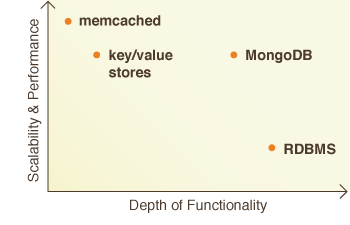
\includegraphics{featuresPerformance.png}}
  \end{center}
\end{frame}

\section[Outline]{}
\begin{frame}
  \MongoLogo
  \tableofcontents
\end{frame}

\section{What is MongoDB?}
\subsection{Document Oriented}
\begin{frame}[fragile]
  \MongoLogo
  \begin{itemize}
    \item Organized into Databases and Collections (like Tables)
    \item Document Oriented
    \item JSON-like (BSON)
    \item Schemaless
    \item Dynamic, Strong Typing
    \item Database can ``reach into'' objects
  \end{itemize}

  \begin{small}
  \begin{verbatim}
db.people.insert({
  _id: "mstearn",
  name: "Mathias Stearn",
  karma: 42,
  active: true,
  birthdate: new Date(517896000000),
  interests: ["MongoDB", "Hadoop", "Üñíçøđĕ"],
  subobject: {foo: "bar"}
});
  \end{verbatim}
  \end{small}

\end{frame}

\subsection{JavaScript Enabled}
\begin{frame}[fragile]
  \MongoLogo
  JavaScript used for:
  \begin{itemize}
    \item Shell and Documentation
    \item (Very) Advanced Queries
    \item ``Group By'' Queries
    \item MapReduce
  \end{itemize}

  \begin{verbatim}
db.users.find({$where: "this.a + this.b >= 42"});
db.posts.group(
  { key: "user"
  , initial: {count:0, comments:0}
  , reduce: function(doc,out){
      out.count++;
      out.comments += doc.comments.length; }
  , finalize: function(out){ 
      out.avg = out.comments / out.count; }
  });
  \end{verbatim}
\end{frame}

\subsection{Fast, Scalable, Available, and Reliable}
\begin{frame}
  \MongoLogo
  \begin{itemize}
  \item Master-Slave replication for Availability and Reliability
    \begin{itemize}
      \item Replica-Pairs support auto-negotiation for master
    \end{itemize}
  \item Auto-Sharding for Horizontal Scalability
    \begin{itemize}
      \item Distributes based on specified field
      \item Currently alpha
    \end{itemize}
  \item MMAP database files to automatically use available RAM
  \item Asynchronous modifications
  \end{itemize}
\end{frame}

\begin{frame}
  \MongoLogo
  \center
  \pgfuseimage{sharding}
\end{frame}

\section{What Makes Mongo Special?}

\subsection{Native Language Integration}

\begin{frame}
  \MongoLogo
  \begin{block}{Official}
    \begin{itemize}
      \item Java/JVM
      \item Python
      \item Ruby
      \item C/C++
      \item Perl
      \item PHP
    \end{itemize}
  \end{block}

  \begin{block}{Community Supported}
    Closure, 
    Scala,
    C\#,
    Haskell,
    Erlang,
    {\it and More}
  \end{block}
\end{frame}

\subsection{Rich Data Types}
\begin{frame}[fragile]
  \MongoLogo
  \begin{block}{JSON}
  \begin{itemize}
    \item String (UTF8)
    \item Double
    \item Object (hash/map/dict)
    \item Array
    \item Bool
    \item Null / Undefined
  \end{itemize}
  \end{block}

  \begin{block}{Extras}
  \begin{itemize}
    \item Date
    \item Int32 / Int64
    \item ObjectID (12 bytes: timestamp + host + pid + counter)
    \item Binary (with type byte)
  \end{itemize}
  \end{block}
\end{frame}

  
\subsection{Atomic Modifiers}
\begin{frame}[fragile]
  \MongoLogo
  \begin{itemize}
    \item \$set
    \item \$inc
    \item \$multiply (soon)
    \item \$push / \$pushAll
    \item \$pull / \$pullAll
  \end{itemize}


    \begin{small}
    \begin{verbatim}
db.posts.update({_id:SOMEID}, {$push:{tags:"mongodb"}})
db.tags.update({_id:"mongodb"}, {$inc:{count:1}},
                      {upsert:true}})
    \end{verbatim}
    \end{small}
\end{frame}

\subsection{Dynamic Queries}

\begin{frame}[fragile]
  \frametitle{Simple}
  \MongoLogo

  \begin{verbatim}
  db.posts.findOne({ user: "mstearn" });

  var cursor = db.posts.find({ user: "mstearn" });
  cursor.forEach(function(){
    doSomething(this.text);
  });
  \end{verbatim}
  
\end{frame}

\begin{frame}[fragile]
  \frametitle{Sorted}
  \MongoLogo

  \begin{verbatim}
  db.posts.find(
    { user: "mstearn" }
  ).sort({timestamp:-1})
  \end{verbatim}
  
\end{frame}
\begin{frame}[fragile]
  \frametitle{Paginated}
  \MongoLogo

  \begin{verbatim}
  db.posts.find(
    { user: "mstearn" }
  ).sort({timestamp:-1}).skip(10).limit(10);
  \end{verbatim}
  
\end{frame}
\begin{frame}[fragile]
  \frametitle{Simple Tag Search}
  \MongoLogo

  \begin{verbatim}
  db.posts.find(
    { user: "mstearn"
    , tags: "mongo"
    }
  ).sort({timestamp:-1}).skip(10).limit(10);
  \end{verbatim}
  
\end{frame}

\begin{frame}[fragile]
  \frametitle{Complex Tag Search}
  \MongoLogo

  \begin{verbatim}
  db.posts.find(
    { user: "mstearn"
    , tags: {$in: ["mongo", "mongodb"]}
    }
  ).sort({timestamp:-1}).skip(10).limit(10);
  \end{verbatim}
  
\end{frame}

\begin{frame}[fragile]
  \frametitle{Nested Objects}
  \MongoLogo

  \begin{verbatim}
  db.posts.find(
    { user: "mstearn"
    , tags: {$in: ["mongo", "mongodb"]}
    , comments.user: "mdirolf"
    }
  ).sort({timestamp:-1}).skip(10).limit(10);
  \end{verbatim}
  
\end{frame}
\begin{frame}[fragile]
  \frametitle{Regular Expressions}
  \MongoLogo

  \begin{verbatim}
  db.posts.find(
    { user: "mstearn"
    , tags: {$in: ["mongo", "mongodb"]}
    , comments.user: "mdirolf"
    , text: /windows/i
    }
  ).sort({timestamp:-1}).skip(10).limit(10);
  \end{verbatim}
  
\end{frame}
\begin{frame}[fragile]
  \frametitle{Ranges}
  \MongoLogo

  \begin{verbatim}
  db.posts.find(
    { user: "mstearn"
    , tags: {$in: ["mongo", "mongodb"]}
    , comments.user: "mdirolf"
    , text: /windows/i
    , points: {$gt: 10, $lt 100}
    }
  ).sort({timestamp:-1}).skip(10).limit(10);
  \end{verbatim}
  
\end{frame}
\begin{frame}[fragile]
  \frametitle{Arbitrary JavaScript}
  \MongoLogo

  \begin{verbatim}
  db.posts.find(
    { user: "mstearn"
    , tags: {$in: ["mongo", "mongodb"]}
    , comments.user: "mdirolf"
    , text: /windows/i
    , points: {$gt: 10, $lt 100}
    , $where: "this.a + this.b >= 42"
    }
  ).sort({timestamp:-1}).skip(10).limit(10);
  \end{verbatim}
\end{frame}


\section{MapReduce}
\subsection{In Mongo}
\begin{frame} [fragile]
  \MongoLogo

  \begin{small}
  \begin{verbatim}
db.posts.mapReduce(
   function() {
     this.comments.forEach(x){
       emit(c.user, 
            {count:1, words:c.words.length}) } }
 , function(key, values){
     for (var i=1; i<values.length; i++){
       values[0].count += values[i].count;
       values[0].words += values[i].words; } }
 , { finalize: function(out){ 
       out.avg = out.words / out.count;
       return out;}
   , query: {posted: {$gt: new Date(2010,0,1)}}
   , out: 'posts.comment_stats'
   }
 });
  \end{verbatim}
  \end{small}
\end{frame}

\section{}
\begin{frame}{Links}
  \MongoLogo
  \begin{itemize}
    \item http://mongo.kylebanker.com (Try mongo in your browser)
    \item http://www.mongodb.org
    \item \#mongodb on irc.freenode.net
    \item mongodb-user on google groups
  \end{itemize}
  \begin{itemize}
    \item mathias@10gen.com
    \item @mathias\_mongo on titter
  \end{itemize}
\end{frame}

\end{document}

% vim: set softtabstop=2
